\documentclass[12pt, a4paper, titlepage]{extarticle}
\usepackage[english]{babel}
\usepackage[utf8]{inputenc}

\usepackage{fontspec}
\newfontfamily\headingfont[]{BerninoSansOffc-Bold.otf}
\newfontfamily\sectionfont[]{BerninoSansOffcSb.otf}
\newfontfamily\subsectionfont[]{BerninoSansOffc.otf}
\newfontfamily\subsubsectionfont[]{freight-text-bold.otf}

\usepackage{titlesec}
\usepackage{titling}
\titleformat*{\section}{\color{hdrie}\LARGE\sectionfont}
\titleformat*{\subsection}{\color{hvier}\Large\subsectionfont}
\titleformat*{\subsubsection}{\color{hdrie}\large\subsubsectionfont}
\renewcommand{\maketitlehooka}{\color{hdrie}\huge\headingfont}

\setmainfont[
 BoldFont={freight-text-bold.otf}, 
 ItalicFont={freight-text-italic.otf}
 ]{freight-text-book.ttf}
 
\usepackage{color}
\definecolor{hdrie}{gray}{0.2}
\definecolor{hvier}{gray}{0.56}
% Specify different font for section headings
\usepackage{fontspec}
% Uncomment the following line to replace the default Latex font with a better readable font for people with dislexia.
%\setmainfont[Ligatures=TeX]{OpenDyslexic-Regular.otf}
\usepackage{hyperref}
\hypersetup{
    colorlinks,
    citecolor=hdrie,
    filecolor=hdrie,
    linkcolor=hdrie,
    urlcolor=hdrie
}

\usepackage{amsmath}

\usepackage{chngcntr}
\counterwithin{figure}{section}

\usepackage{hologo}
\newcommand*{\bfrac}[2]{\genfrac{}{}{0pt}{}{#1}{#2}}

\begin{document}
	\title{Summary Principles of Economics for Scientists}
	\color{hdrie}
	\author{Michael Vanderstuyft \and Thor Galle \and Joppe Geluykens}
	\abstract{\begin{center}
	First draft of a summary of the first 3 parts of this course, based on the Google Doc created by Thor and Michael (thank you guys so much!) and the slides of the course as available on Toledo.\\
	This \hologo{LaTeX} document is formatted in the style of the \href{http://www.medium.com}{Medium blog/publishing platform}. Template created by Joppe.\\
	To be completed.
	\end{center}}
	\date{}
	\maketitle
	
	\tableofcontents
	\pagebreak
	
	\section{Introduction}
	\subsection{Course material}
	Textbook is freely available on the web.
	
	McAfee, R. Preston \textit{Introduction to Economic Analysis}\\
	\url{https://en.wikipedia.org/wiki/Introduction_to_Economic_Analysis}\\
	Download book: \url{http://www.muhlenberg.edu/iea/}\\
	May be worth looking at: \url{http://www.mcafee.cc/Classes/Ec11/}
	
	\subsection{Exam}
	
	\begin{itemize}
		\item Don't memorise too much,
		\item Make all exercises\\
				Exam will exist mostly out of variations on the exercise sessions.
		\item Be able to reproduce deductions from the lectures,
		\item If not seen in lecture, but covered in book; just reading suffices.
		\item 2nd part not to know: spillovers
	\end{itemize}
	
	Information \& Innovation:
	\begin{itemize}
	\item one part exercises like from the excercise sessions
	\item another  part concepts, understanding the slides is enough
	\end{itemize}
	
	\pagebreak
	\section{Demand \& Supply}
	Chapters 2 and 3.
	\subsection{Demand}
	
	Demand drives market prices.\\
	Market independence $\Leftrightarrow$ Governement involvement = important\\
	
	\begin{description}
		\item[Diminishing marginal value] willingness to pay ($v(q)$) for the good decreases when the quantity increases.
		\item[Demand] quantity you are willing to consume at that particular price of a good.
		\item[Economic gain = consumer surplus] difference between $v(q)$ and the price actually paid. 
	\end{description}
	
	\begin{figure}[h]
	\centering
		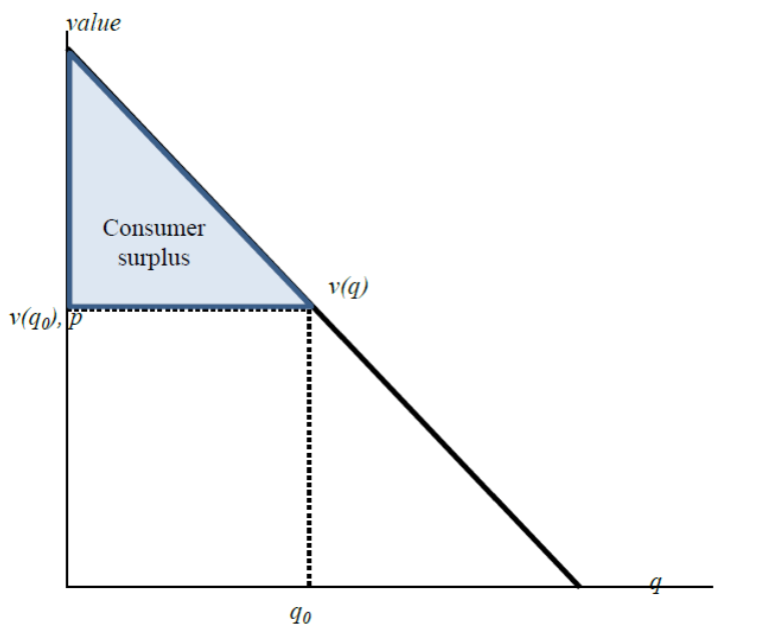
\includegraphics[width=8cm]{consumersurplus}
		\caption{You purchase a good until your demand at $q_0$ is smaller than the price you have to pay.\label{imgConsumerSurplus}}
	\end{figure}
	Demand depends on utility: consumer surplus.\\
	\[u'(q) = v(q) \]
	$gain = u(q) - qp$ \\
	1$^{st}$\ order condition $= u'(q) = p$\\
	
	\begin{equation}
		\begin{gathered}
			CS = \int_0^{q_0}(u'(q) - p)dq = \int_0^{q_0}(v(q) - p)dq, \text{ see figure \ref{imgConsumerSurplus}}
		\end{gathered}
	\end{equation}
	Demand is defined by:
	
	\begin{itemize}
		\item Income
		\begin{description}
			\item[Normal goods] demand for some goods increases with income (Porsches, yachts, ...).
			\item[Inferior goods] demand for other goods may decrease with income (bus tickets, ...).
		\end{description}
		\item Complementarity
		\begin{description}
			\item[Complements] goods that must be consumed jointly with other goods (tables \& chairs, hardware \& software, cars \& gas, ...). 
			\item[Substitutes] goods that replace other goods (French fries \& sushi, beer \& marijuana, ...).
		\end{description}
		\item Fashion
		\begin{description}
			\item Some goods are in strong demand in one year and not so much in another year without any changes in incomes or complementarity.
		\end{description}
	\end{itemize}
	
	\textbf{Demand drives supply. Never the other way around!}
	
	\subsection{Supply}
	
	Low prices $\Rightarrow$ little production.\\
	High prices $\Rightarrow$ more and more production. \\
	Result: supply function is upward sloping. 
	(See figure \ref{imgPriceSupplyProfit}.)\\
	
	\begin{description}
		\item[Supply function] function that gives the quantity produced as a function of the price. 
	\end{description}
	\begin{figure}[h]
	\centering
		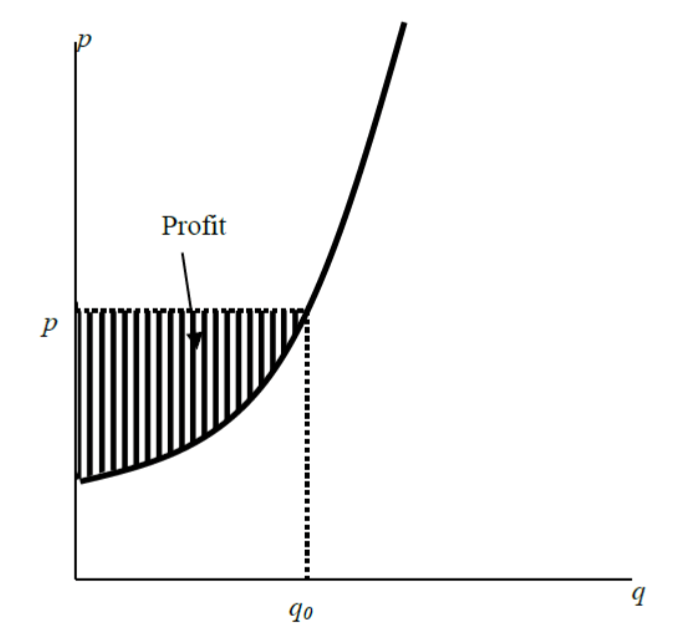
\includegraphics[width=8cm]{pricesupplyprofit}
		\caption{The company's profit is given by the area between price and supply curve. \label{imgPriceSupplyProfit}}
	\end{figure}
	Calculating the supply function:\\
	\begin{equation}
		\begin{gathered}
			\text{profit}\ \pi = pq - c(q), \\ 
			\text{optimal quantity implicitly defined by first-order condition}\ p = c'(q),\\
			c\ \text{is convex, optimal quantity increases in good's price},\\
			\text{at a given price}\ p, \text{profit maximizing quantity is}\ q_0,\\
			\text{Total profit} = \pi = pq_0 - c(q_0) = \int_0^{q_0}(p - c'(q))dq.
		\end{gathered}
	\end{equation}
	\\
	Supply is defined by input prices:
	
	\begin{description}
		\item[Capital] the price of capital is the interest rate,
		\item[Labor] the price of labor is the worker's wage.
	\end{description}
	$\Rightarrow$ These factors shift the supply curve upwards (raise in input prices) or downwards (decrease in input prices).\\
	
	\begin{description}
		\item[Demand exceeds supply = shortage] The prices will go up, and bigger supply can be given. Upwards pressure on prices.\\
		E.g.: there is a firm that wants to produce 100 cars at price p \& there are 160 people who want to purchase a car.
		\item[Supply exceeds demand = surplus] To sell all the goods, the producers lower the price. Downwards pressure on prices.
	\end{description}
	See figure \ref{imgEquilibriumShortageSurplus}.
	
	\subsection{Market Equilibrium}
	
	\begin{description}
		\item[Market equilibrium] equilibrium price equalizes demand and supply.
		\item[Pareto-efficient] prices are not really negotiatable; maximizes gains from trade.\\
		Impossible to make any one individual better off without making at least one individual worse off.
	\end{description}
	
	\begin{figure}[h]
	\centering
		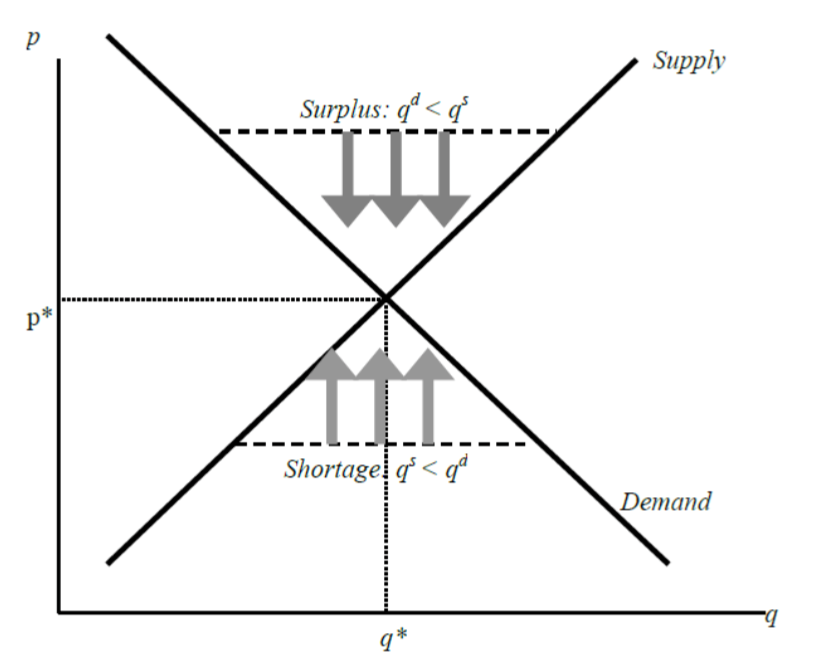
\includegraphics[width=8cm]{EquilibriumShortageSurplus}
		\caption{Market equilibrium, shortage and surplus. \label{imgEquilibriumShortageSurplus}}	
	\end{figure}
	
	\subsection{Elasticity}
	
	What drives market demand and supply?
	
	\begin{description}
		\item[Price elasticity of demand] by how many percent demand decreases if the price goes up by one percent. 
	\end{description}
	
	\begin{equation}
		\begin{gathered}
			\varepsilon = -\frac{p}{x}\frac{dx}{dp} = -\frac{p}{x(p)}x'(p), \\ \text{with $x(p)$ the demand function,} \\ \text{$\varepsilon$ is independent of the change in x (expressed in \% and unit free.}
		\end{gathered}
	\end{equation}
	
	\begin{description}
		\item[$\varepsilon < 1$] demand decreases by \textbf{less} than one percent if the price increases by one percent. Demand is \textit{inelastic} (\textbf{increase in total revenue}). 
		\item[$\varepsilon > 1$] demand decreases by \textbf{more} than one percent if the price increases by one percent. Demand is \textit{elastic} (\textbf{decrease in total revenue}).
		\item[$\varepsilon = 1$] total revenue stays the same 
	\end{description}
	Complements have a small elasticity.\\
	Substitutes have a large elasticity. (usually)\\
	\\
	Goods can have both a high and low elasticity.\\
	\textit{E.g.:} airline travel
	
	\begin{itemize}
		\item \textbf{short-run} (last minute booking): low elasticity, you have to buy the ticket.
		\item \textbf{long-run} (usually vacation travel): high elasticity, you can go somewhere else, or you can go by other means of transport. 
	\end{itemize}
	
	\begin{figure}[h]
	\centering
		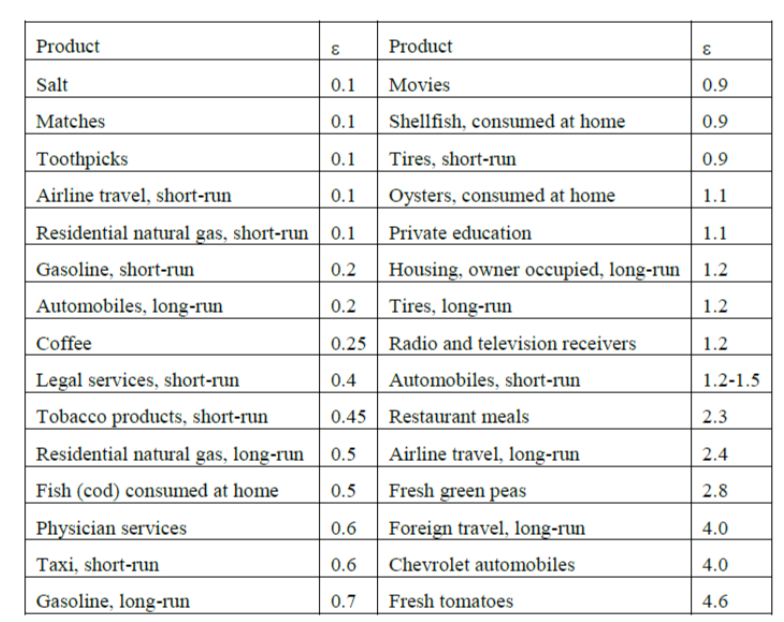
\includegraphics{ElasticityTable}
		\caption{Examples of price elasticities for different goods. \label{imgElasticityTable}}
	\end{figure}

	\pagebreak
	\section{Government interventions}
	Chapters 5, 7 and 8.\\
	The discussion on `Government interventions' as seen in class is a simple model that's not complete. 
	It could therefore give wrong results when applied to a real world situation.
	
	It doesn't matter (in most cases) whether the buyer or seller pays the tax. 
	If buyer (seller) pays tax, this reduces willingness to pay (produce) for any given unit by the amount of tax, thus shifting down the demand (supply) curve by the amount of the tax. 
	(See figure \ref{imgTaxation}.)
	\begin{figure}[h]
	\centering
		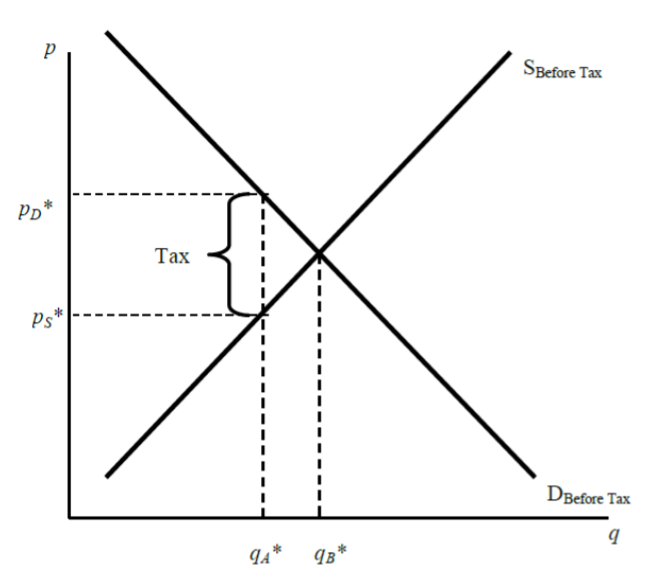
\includegraphics[width=8cm]{Taxation}
		\caption{The equivalence between consumer or producer paying a tax. \label{imgTaxation}}	
	\end{figure}
	\begin{equation}
		\begin{gathered}
			\text{welfare} = \text{CS} + \text{supplier profits}\ (?)
		\end{gathered}
	\end{equation}
	\begin{description}
		\item[Dead weight loss] reduction of quantity traded due to taxation. 
		Does not comprise tax revenues, as these can be used by the government.\\
		$\Rightarrow$ loss of welfare.
	\end{description}
	
	\subsection{Tax Incidence}
	\begin{description}
		\item[Tax incidence = tax burden] by how much quantity, price and welfare fall when a tax is imposed.  
	\end{description}
	Depends on $\varepsilon$ (price elasticity of demand) and $\eta$ (price elasticity of supply).\\
	Suppose total demand is given by $q_d(p) = ap^{-\varepsilon}$ and supply by $q_s(p) = bp^\eta$.\\
	Market equilibrium price without tax $\Rightarrow$ $q_d(p) = q_s(p) \Leftrightarrow ap^{-\varepsilon} = bp^\eta$.\\
	
	Government requests tax $t$ on the value of the good so buyer's price becomes
	\[p_b = (1 + t)p_s \]
	Buyer's equilibrium price:
	\[p_b^* = (\frac{a}{b})^{\frac{1}{\varepsilon + \eta}}(1 + t)^{\frac{\eta}{\varepsilon + \eta}} \]
	Seller's equilibrium price:
	\[p_s^* = (\frac{a}{b})^{\frac{1}{\varepsilon + \eta}}(1 + t)^{-\frac{\eta}{\varepsilon + \eta}} \]
	Equilibrium quantity:
	\[q^* = a^{\frac{\eta}{\varepsilon + \eta}}b^{\frac{\varepsilon}{\varepsilon + \eta}}(1 + t)^{-\frac{\varepsilon\eta}{\varepsilon + \eta}} \]
	
	Convenient goods to request tax on are goods with inelastic demand or supply, resulting in small dead weight loss, because the sold quantity stays almost equal.\\
	If both demand and supply are elastic, than the loss of trade is huge.
	With small tax the ``dead weight loss" is small as well.
	\\
	$v(q) = p$ at the consumer's demand curve.\\
	We can therefore rewrite \textbf{price elasticity of demand} as:
	\begin{equation}
		\begin{gathered}
			\varepsilon = -\frac{p}{q}\frac{dq}{dp} = -\frac{v(q)}{q}\frac{1}{v'(q)} = -\frac{v(q)}{qv'(q)}.
		\end{gathered}
	\end{equation}
	Same for \textbf{supply} ($c(q) = p$):
	\begin{equation}
		\begin{gathered}
			\eta = \frac{c(q)}{qc'(q)}.
		\end{gathered}
	\end{equation}
	In equilibrium:
	
	\begin{equation}
		\begin{gathered}
			p_b^* = v(q^*) = (1 + t)c(q^*) = p_s^*.
		\end{gathered}
	\end{equation}
	From implicit differentiation we get that (must be able to derive this on your own):
	
	\begin{equation}
		\begin{gathered}
			\frac{dq^*}{dt} = -\frac{q^*\varepsilon\eta}{(1 + t)(\varepsilon + \eta}.
		\end{gathered}
	\end{equation}
	Total tax revenue:
	
	\begin{equation}
		\begin{gathered}
			T = tp^*q^* = tc(q^*)q^*.
		\end{gathered}
	\end{equation}
	From this we calculate:
	
	\begin{equation}
		\begin{gathered}
			\frac{dT}{dt} = c(q^*)q^* + t\left[c(q^*)\frac{dq*}{dt} + c'(q*)\frac{dq^*}{dt}q^* \right]\\
			= ... = \frac{c(q^*)q^*}{(1 + t)(\varepsilon + \eta)}(\varepsilon + \eta - t\eta(\varepsilon - 1)).
		\end{gathered}
	\end{equation}
	Total gains from trade ($GFT$):
	
	\begin{equation}
		\begin{gathered}
			GFT = \int_0^{q^*}(v(q) - c(q))dq.
		\end{gathered}
	\end{equation}
	Calculating how $GFT$ changes when increasing tax revenue:
	
	\begin{equation}
		\begin{gathered}
			\frac{dGFT}{dT} = \frac{\frac{dGFT}{dt}}{\frac{dT}{dt}} = \frac{(v(q^*) - c(q^*))\frac{dq^*}{dt}}{\frac{c(q^*)q^*}{(1 + t)(\varepsilon + \eta)}(\varepsilon + \eta - t\eta(\varepsilon - 1))}\\
			= ... = -\frac{t\varepsilon\eta}{\varepsilon + \eta - t\eta(\varepsilon - 1)}.
		\end{gathered}
	\end{equation}
	See full derivation in Google Doc\\ \url{https://docs.google.com/document/d/1y5xPIq8Yxbr4ARFs_TkBi8gyEHahunEXqdhahRlIDc0/} \\
	
	Thus, marginal drop in GFT small for small taxes $t$ and at least one elasticity ($\varepsilon$ or $\eta$) small.
	
	\subsection{Price Floors and Ceilings}
	\begin{description}
		\item[Price floor] government may impose a minimum wage.\\
		\textit{Result:} More people unemployed (big supply, low demand $\Rightarrow$ wasted production, units produced that aren't consumed).\\ Welfare is lost (See figure \ref{imgPriceFloor}, note that this is minimal loss: producers with relatively high production cost can sell, which makes more efficient producers lose customers.)
		\item[Price ceiling] government may choose a maximum price. (roaming fees)\\
		\textit{Result:} If price ceiling below equilibrium price, there is shortage.\\ (See figure \ref{imgPriceCeiling}, again minimal loss.) People with most gain don't necessarily get priority over others. \\ People with willingness to pay below the original equilibrium price can acquire the good.
	\end{description}
	\begin{figure}[h]
	\centering
		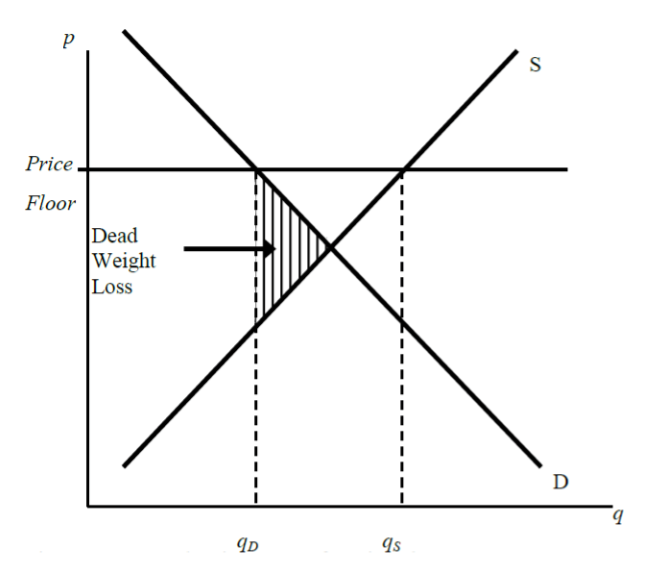
\includegraphics[width=8cm]{PriceFloor}	
		\caption{Welfare loss with imposing price floor. \label{imgPriceFloor}}
	\end{figure}
	\begin{figure}[h]
	\centering
		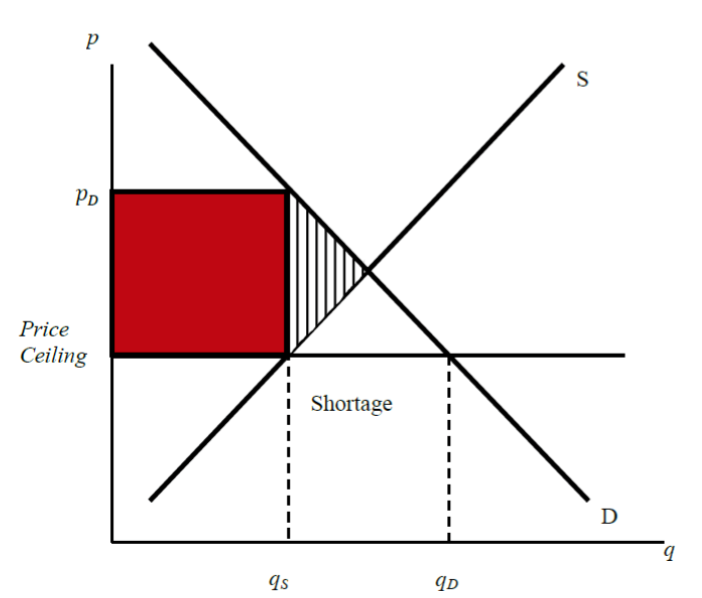
\includegraphics[width=8cm]{PriceCeiling}
		\caption{Welfare loss with imposing price ceiling. \label{imgPriceCeiling}}
	\end{figure}
	
	Imposing a ceiling can result in ``costless discrimination", in which one discriminates a minority because it will not cause revenue losses.\\
	This is a paradox in the ``justice" argument, the reason to impose such type of price.
	
	\subsection{Externalities}
	\begin{description}
		\item[Externality] the welfare of a passive 3$^{th}$ party can be affected by a transaction.\\
		May be a justification for government interventions. (Nice roads, healthcare, ... due to taxes.)
		\begin{itemize}
			\item \textbf{negative example:} global warming.\\
			Our pollution doesn't hurt us as much as the earth as a whole.\\
			\item \textbf{positive example:} vaccinations.\\
			If one takes a vaccinations, she cannot transmit the illness to another 3$^{th}$ party.\\
		\end{itemize}
	\end{description}
	\begin{figure}[h]
	\centering
		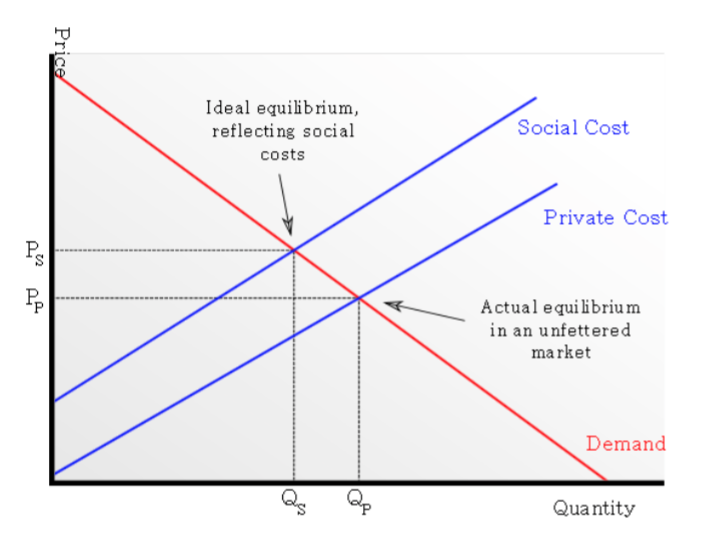
\includegraphics[width=8cm]{Externalities}
		\caption{The effects of externalities on the cost and market equilibrium. \label{imgEffectsOnProductionCostExternalities}}
	\end{figure}
	\begin{figure}[h]
	\centering
		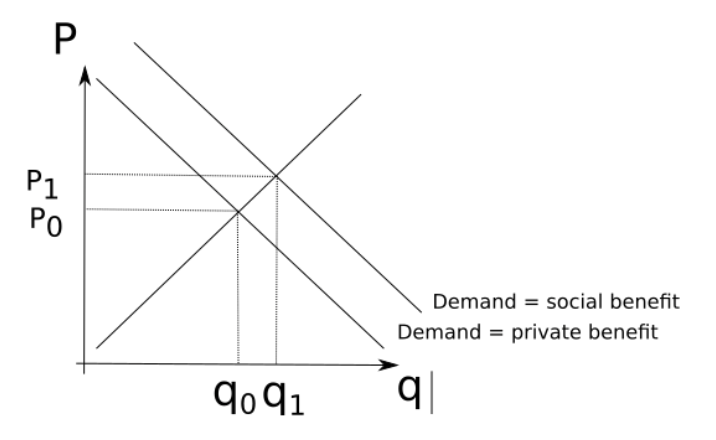
\includegraphics[width=8cm]{ConsumptionExternalities}
		\caption{The effects of externalities on the consumption and market equilibrium. \label{imgEffectsOnConsumptionExternalities}}
	\end{figure}
	
	Externalities are very common, a completely private parket is rare.\\
	Market mechanism typically leads to inefficient results when externalities are present.\\
	\\
	Impact of externalities:
	\begin{itemize}
		\item Negative (see figure \ref{imgEffectsOnProductionCostExternalities}):
			\begin{itemize}
				\item People don't take externality into account. (Only private cost taken into account.)
				\item Negative impact of their production/consumption affects mostly other people (earth) and future generations.
					\begin{itemize}
						\item Every product produced adds social cost to the image. (Cost of society.)
						\item These costs are not taken into account, because of the economy being selfish.
					\end{itemize}
				\item $\Rightarrow$ private cost of production $<$ social costs of production (quantity of production too high, from social POV, see figure \ref{imgEffectsOnProductionCostExternalities}.)
			\end{itemize}
		\item Positive (see figure \ref{imgEffectsOnConsumptionExternalities}):
			\begin{itemize}
				\item $\Rightarrow$ private benefits of consumption $<$ social benefits of consumption (level of consumption too low, from social POV, see figure \ref{imgEffectsOnConsumptionExternalities}.)
			\end{itemize}
	\end{itemize}
	
	\subsubsection{Solutions to Inefficient Allocations in Markets}
	
	Externalities lead to inefficient allocations in markets.\\
	There are 3 solution mechanisms: taxes, quotas and negotiations.
	\subsubsection*{Pigouvian tax}
	We consider a negative externality: ``a mill pollutes a river and thereby reduces the welfare of a bunch of fishermen".
	
	Taxing the production of the good increases the costs for the mill and hence reduces production. There exists a level of taxes that leads to the social optimum. (See figure \ref{imgPigouvianTax}.)
	\begin{figure}[h]
	\centering
		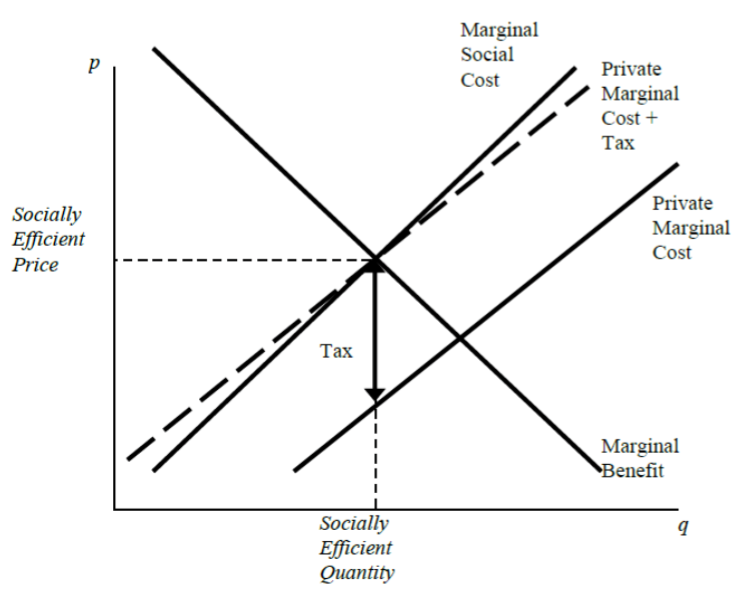
\includegraphics[width=8cm]{PigouvianTax}
		\caption{Graphical representation of the Pigouvian tax. \label{imgPigouvianTax}}
	\end{figure}
	
	The problem of taxes is that government usually doesn't know mill's cost structure, neither true welfare loss of fishermen. Hence, unclear what is optimal level of taxes.
	
	Mill has no incentive to report true cost structure. Instead, reports cost structure that reduces tax as much as possible. Similarly, fishermen have incentive to report inflated welfare losses.
	
	Regulation of large firms to counter externalities is a big topic in economics, but N/A for this course.\\
	\\
	Taxes make no death weight loss with externality.\\
	\\
	Figuring social marginal cost very debatable
	\begin{itemize}
		\item How much worth is tomorrow for us today?
		\item Government does not have the correct info, involved parties often not honest in order to maximize (current) gain.
	\end{itemize}
	
	\subsubsection*{Quotas}
	Government wants to increase consumption/production of goods that create positive externalities.
	
	An alternative to the Pigouvian tax: set a quota, a limit on the activity. Quotas can be maxima or minima (on produced quantity), depending on whether the activity generates negative or positive externalities.
	
	Maximum quotas are used, for example, to limit pollution (such as carbon emissions).
	
	Minimum quotas are much more common regulatory strategy for dealing with externalities than taxes or subsidies.
	
	Like taxes, not clear how large they should be and who should get them. (e.g.: the right to pollute)\\
	\\
	One solution:
	\begin{itemize}
		\item Make quotas tradeable (e.g.: carbon emission trading)
		\begin{itemize}
			\item Producers who easily avoid pollution sell their quotas to producers for whom it's costly to avoid pollution.
			\item Allocation of quotas will be pareto-efficient; quotas will go to the producers who benefit most from them.
			\item If society has high valuation for reduction of pollution, government can purchase quotas and not use them.
		\end{itemize}
	\end{itemize}
	
	\subsubsection*{Negotiating/bargaining}
	`Coase' argued that bargaining can solve problems of externalities, and that real problem is ill-defined property rights (Wha has the right to pollute? Does your neighbour have the right to play loud music?)
	
	``Coasian Bargaining" may work well in small groups; less successful when many parties involved (recurrent climate negotiations).
	
	\subsection{Public Goods}
	Special kind of goods with positive externalities.\\
	Two properties:
	\begin{enumerate}
		\item \textbf{Nonexcludability}: difficult (impossible) to exlude people from using the good
		\item \textbf{Nonrivalry}: many people can use the good simultaneously
	\end{enumerate}
	Examples:
	\begin{itemize}
		\item National defense
		\item Scientific publications (without patents) 
		\item Public parks
		\item Highways
	\end{itemize}
	For last two, nonrivalry has limits. Nonrivalry as long as few people are using the good, rivalry when too many individuals using the good.
	
	Typically, provision of public good through markets too low; like for consumption goods with positive externalities, too little consumed in equilibrium.
	
	Lack of incentive for individuals to contribute to social good = \textbf{free-rider problem}. E.g.: writing paper in group, waiting for others to write as much as possible.
	
	All individuals of a community agree on optimal provision of a public good $\Rightarrow$ paid by government with taxation.\\
	Else, benefit goes from people not using good to people using good.
	
	Possible solution, people `vote with their feet'; different areas with different types of provided public goods. People move to place they like most concerning distribution of taxes vs. amount of public goods.
	
	\pagebreak
	\section{Producer theory}
	Chapters 9, 10 and 11. (Only need to know as detailed as the slides, not the book.)
	\begin{itemize}
		\item How do firms react to price changes
		\item Investments
		\item V = future value, A = asset (also called principal), r = interest rate, t = amount of periods (typically years), $A = \frac{V}{(1+r)^t}$ 
		\item $PDV = \frac{1200}{(1+r)^5}$, (slide 27/41)
		\item NPV of the project "buy a Blu-ray player immediately"? 
		\[ NPV = -450 + 50 + 0.75.\frac{1}{1+0.05}.\frac{50}{0.05} \cong 314 \]
		\item NPV of the project "buy a HD DVD player immediately"? 
		\[ NPV = -400 + 50 + 0.25.\frac{1}{1+0.05}.\frac{50}{0.05} \cong -112 \]
		\item NPV of the project "wait for one period"?
		\begin{equation}
		    \begin{gathered}
		        NPV = \\ \frac{1}{1+0.05}\left[0.75\left(-450 + \frac{50}{0.05}\right) + 0.25\left(-400 + \frac{50}{0.05}\right)\right] \\ \cong 538
		    \end{gathered}
		\end{equation}
		\\
		\item einde slides 3. Producer Theory 41/41
	\end{itemize}
	
	\section{Consumer Theory}
	Chapter 12.
	\begin{itemize}
		\item H12 in boek
		\item einde les, slide 18/29 4. Consumer Theory
		\item slide 16/29: s.t. = ``subject to"
	\end{itemize}
	
	\begin{figure}[h]
	\centering
	    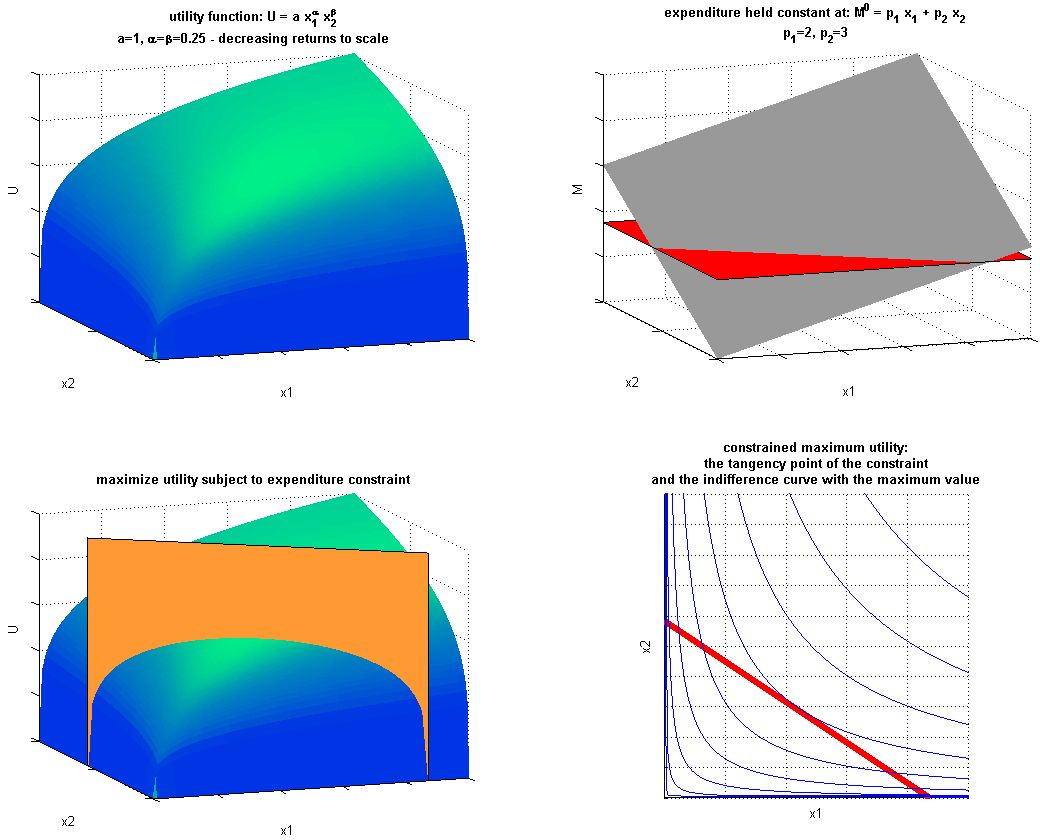
\includegraphics[width=8cm]{utility_drs_cr.jpg}
	    \caption{Maximization of utility function \label{fig:imgMaxUtility}}
	\end{figure}
	In the consumption optimum you pick the point on the budget line where you can reach the highest possible utility.\\ \newline
	What happens when the price ratio changes?\\
	\begin{itemize}
	\item {One good all consumers need increases price. \\ using this product makes it less attractive (in comparison with other things) \textbf{substitution effect}}
	\item{It's the same as becoming poorer, because you cannot buy a big amount of the product anymore. \textbf{income effects}}
	\item{How can we distinguish the 2 effects above.}
	\begin{itemize}
	\item {new consumption bundle line flattens out when one product gets more expensive}
	\item{When prices go up, we give the consumer more money, until the consumer can still buy the same amount (have the same level of utility) as he would with the old consumption bundles. (compensated demand) \textbf{pure substitution effect}}
	\end{itemize}
	\end{itemize}
	
	\begin{figure}[htp]
	\centering
	    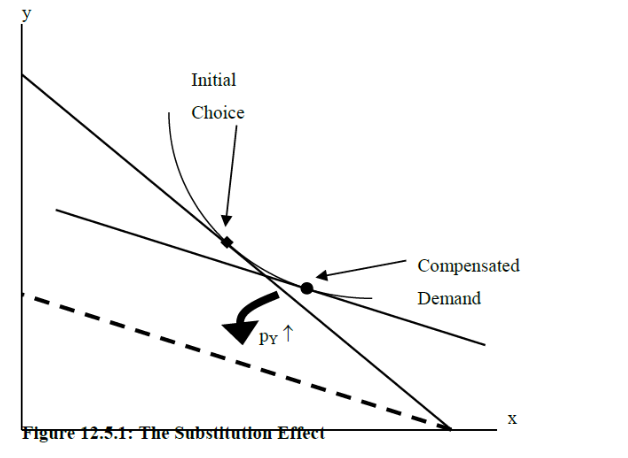
\includegraphics[width=8cm]{utility.png}
	    \caption{new consumption bundles graph\label{fig:utility}}
	\end{figure}
	\begin{figure}[htp]
	\centering
	    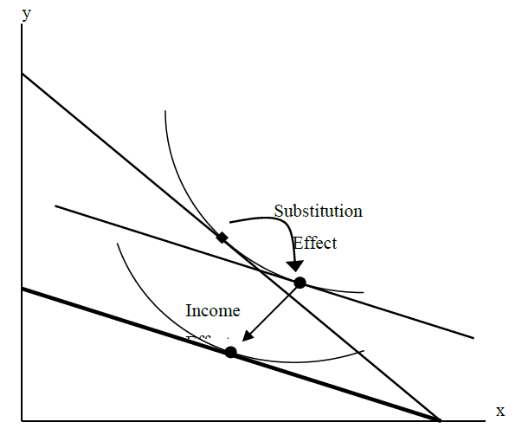
\includegraphics[width=8cm]{substitution_effect.png}
	    \caption{income effect\label{fig:substitution_effect}}
	\end{figure}
	\begin{itemize}
	\item{\textbf{substitution effect} makes you buy more of other things}
	\item{\textbf{income effect} makes the change in the consumption negative}
	\end{itemize}
	It is possible to get more items sold with bigger price (theoretically)\\
	\begin{figure}[htp]
	\centering
	    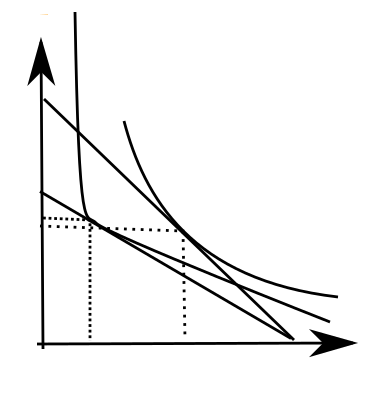
\includegraphics[width=8cm]{price_increase_quantity_increase.png}
	    \caption{selling bigger quantity when price increases\label{fig:pricequantum}}
	\end{figure}
	
	Examples of this are status-symbols like very expensive watches and cars.
	
	\subsection{Engel curves}
	
	\subsubsection{Engel curve for Cobb-Douglas utility function}
	\[ \mathcal{L} = Ax^{\alpha}y^{1-\alpha} - \lambda(p_xX+p_yY - M) \]
	
	
	$\dfrac{\partial L}{\partial x} = \alpha Ax^{\alpha-1}y^{1-\alpha}- \lambda p_x = 0$ (1)\\
	
	$\dfrac{\partial L}{\partial y} = (1-\alpha)Ax^\alpha y^{-\alpha} - \lambda p_y = 0$ (2)\\
	
	$\dfrac{(1)}{(2)} \Rightarrow \dfrac{\alpha y}{(1-\alpha)x}= \dfrac{p_x}{p_y} \Rightarrow y = \dfrac{1-\alpha}{\alpha} \cdot \dfrac{p_x}{p_y}x$\\
	
	If you get richer, you continue consuming more good.
	\textbf{not true}, because: you will shift your consumption to a completely different kind of good (eventually).
	
	Goods that you stop purchasing once you get richer are \textbf{inferior goods} the new goods bought are \textbf{superior goods}.
	
	In a model of two goods, it is not possible for both to be inferior, income has to be spent somehow.
	
	\section{Monopoly I}
	Chapter 15 (more information on the slides).
	
	\subsection{Class 5 - notes}
	\begin{itemize}
	\item Most markets firms enjoy some market power.
	\begin{itemize}
	\item when having market power, a firm can influence the price by varying the quantity produced (iPhones)
	\end{itemize}
	\item mostly multiple firms have a part of the market power. (e.g., apple and samsung for smartphones)
	\item What can the government do if this monopoly reduces the total welfare.
	\end{itemize}
	
	\subsubsection{Profit maximization}
	\begin{itemize}
	\item In the case of a monopoly, the price $p(q)$ depends on the quantity $q$. This is a difference with perfect competition.
    \item $\dfrac{d \pi (q)}{dq}= p'(q)q + p(q) - c'(q) = c$
    
    \begin{itemize}
    \item if q increases, price decreases
    \item if q increases revenue increases
    \item if q increases costs increase
    \end{itemize}
    \item $\bfrac{max}{q}(50-4q)q-2q$ \\ $\dfrac{\partial}{\partial q} = 50 - 4q - 4q -2 = 0\\ \Rightarrow q^n = 6 \\ \Rightarrow p^m = 50 - 4q^m = 26 \\
    \pi^m = q^m p^m - c(q^m) = 144$
	\item Lerner index
	\begin{itemize}
	\item can range between 0 and 1
	\item 0 is perfectly competitive market
	\item 1 you own the market
	\item $\dfrac{p^m - c'(q^m)}{p^m}$
	\item Even when having big data, a firm can not always estimate the optimal marker. E.g., Amazon conducted a price variation experiment to determine the demand, but it resulted in a lot of problems (unhappy consumers).
	\end{itemize}
	\item Not the size of a company matters, but the firms ability to charge a price over marginal cost.
	\end{itemize}
	
	
	\subsubsection{Sources of Market Power}
	
	\begin{itemize}
	\item Where does market power come from?
    	\begin{itemize}
    	\item natural monopoly: huge investment costs in the beginning. from then the marginal cost lowers for every additional quantity produced. (The more you produce the cheaper the cost for an individual product) E.g., telecommunication. (placing of the net is very expensive) 
        	\begin{itemize}
        	\item a firm can throw the competitor out of the market by reducing the cost below the average cost of the other, and attracting all their customers. Now the other company cannot produce at the same price anymore (therefore they needed the customers).
        	\end{itemize}
    	\item If Cuba becomes a capital try to invest into a natural monopoly
    	\item Switching costs: it is very hard to build a firm like Facebook if a firm like that already exists. (try to make it as difficult as possible for your clients to switch)
    	\item Product differentiation: eg. cars have a consumer loyalty.
    	\item Product needed by all producers, buy all competitors from the market by purchasing the firms that 
    	\item Government regulation examples Taxi license, copyrights
    	\end{itemize}
    \end{itemize}
	
	\subsubsection{Comparative Statistics (Market Changes)}
	
	\subsubsection{Welfare Implications (Winners and Losers)}
	\begin{itemize}
    \item If there is winners in the market power, there must also be losers
        \begin{itemize}
        \item market power benefit the firm, but not the consumers 
        \item monopoly: $\pi = (1000 - 5q) q - 200 q \Rightarrow q^m = 80, p^m= 600$
        \item perfect competition: $1000 - 5q = 1200 \Rightarrow q^c=160, p^c = 200$
        \begin{figure}[htp]
	\centering
	    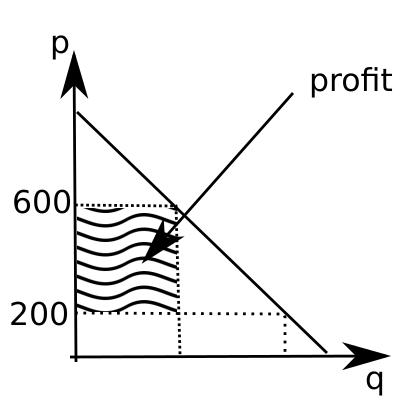
\includegraphics[width=8cm]{monopoly_profit.png}
	    \caption{monopolist surplus\label{fig:monopoly_profit}}
	\end{figure}
	    \item monopoly consumer surplus is $\dfrac12 (1000 - 600)80 = 1600$
	    \item perfect competition consumer surplus is $\dfrac12 (1000 - 200)160 = 64000$
	    \item \textuf{total welfare}\\ monopoly: total surplus is 16000 (that is cs) + (600 - 200) 80 (that is $\pi^m$) = 48000
	    \item perfect competition: total surplus is 64000
        \end{itemize}
    \item market-power does 2 things
    \begin{itemize}
    \item replaces costumer surplus to profit
    \item reduces total welfare
    \end{itemize}
    \end{itemize}
	
	\subsubsection{Regulation, Antitrust and Innovation}
	\begin{itemize}
	\item Government tries to increase the total welfare by setting price ceilings
	\item problem: the government does not have the cost structure of the firms
	\item Antitrust regulation, detect if there is illegal coalitions between firms. 
	\begin{itemize}
	\item cartels can be detected mostly by phone calls and ... .
	\item when detected, huge fines have to be payed.
	\end{itemize}
	\item when is market power a good thing
	\begin{itemize}
	\item when high technology products are produced, the price of research is very high
	\item but the price of production are very low. 
	\item market power gives the opportunity to regain the loss made for the research
	\end{itemize}
	
	\end{itemize}
	
	\section{Monopoly II: Price Discrimination}
	Chapter 15.
	
	\begin{description}
	\item[arbitrage] a customer that paid a lower price (because of price discrimination) will sell it to a customer with a higher willingness to pay, assumed nonexistent here
	\item[perfect price discrimination] everyone pays exactly his willingness to pay. (The monopolist can charge everyone with a different price)
	\end{description}
	\begin{itemize}
	\item the monopolist gets all the gains of trade
	\item it is efficient, though it may not be "fair"
	\item not realistic, it can only be reached by a very persuasive seller who gets every customer to pay their individual willingness to pay.
	\end{itemize}
	\begin{figure}[htp]
	\centering
	    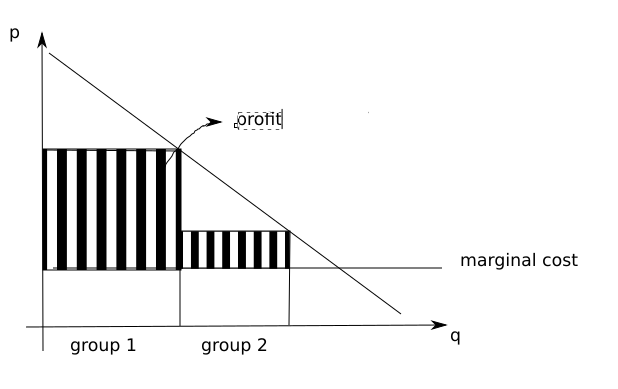
\includegraphics[width=8cm]{monopoly2prices.png}
	    \caption{monopolist can set 2 prices for different groups of consumers\label{fig:monopoly2prises}}
	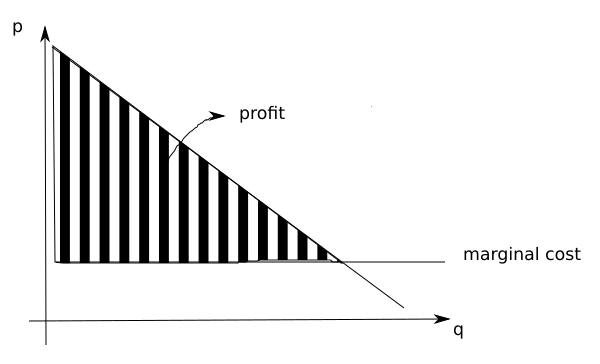
\includegraphics[width=8cm]{perfect_price_discrimination.png}
	    \caption{monopolist can get all gains of trade\label{fig:monopoly_perfect_price_discrimination}}
	\end{figure}
   
	    
	\subsection{Segmentation}
	\begin{description}
	\item[segmentation]dividing into two price/consumer groups: 
	\end{description}
	$\\\dfrac{\partial \pi(q_1, q_2)}{\partial q_1} = p'_1(q_1)q_1 + p_1(q_1) - c'(q_1+q_2) = 0\\
	\dfrac{\partial \pi(q_1, q_2)}{\partial q_2} = p'_2(q_2)q_2 + p_2(q_2) - c'(q_1+q_2) = 0\\$
	\newline
	$q_T = 1700 - 5p_T \Rightarrow p_T = 340-\dfrac{1}{5}q_T\\
	q_L = 2400 - 10p_L \Rightarrow p_L = 240 - \dfrac{1}{10}q_L\\$
	\newline
	$\pi = (340 - \dfrac{1}{5} q_T) q_T + (240 - \dfrac{1}{10} q_L) q_L - 100(q_T + q_L) $
	$\dfrac{\partial \pi}}{\partial q_T}= 340 - \dfrac{2}{3} q_T - 100 = 0 \Rightarrow q_T 600\\
	\dfrac{\partial \pi}{\partial q_L}= 240 - \dfrac{1}{5}q_L-100 = 0 \Rightarrow q = 700\\$
	\newline
	\begin{itemize}
	\item price discrimination over time: price goes down over time. Price starts high, but becomes lower over time.
	\begin{itemize}
	\item the middle buyer will wait to buy at lower price
	\item the producer keeps the price high for a very long time
	\end{itemize}
	\item generally the government prohibits price discrimination on gender (life insurance might make use of this characteristic, average life time differs between genders)
	\end{itemize}
	
	\subsection{Indirect price discrimination}
	\begin{itemize}
	\item based on characteristics that the monopolist can not see
    	\begin{itemize}
    	\item e.g. mobile phone providers
    	\item different kinds of consumers can get different contracts
    	\end{itemize}
	\item consumer can select himself what price he will pay (according to the quantity that he wants).
    \item difficulty: the contracts/menu's should be chosen wisely
        \begin{itemize}
        \item the combination of price vs service of every contract must attract enough customers
        \item if the high price is to high, nobody takes it
        \item if it is to low, than everyone will take it
        \end{itemize}
	\item defining these prices are no part of this course
	\item incentive compatible: match consumer's incentives with appropriate contracts 
	\end{itemize}
	
	\subsection{Bundle products}
	\begin{itemize}
	\item bundle products: don't give 1 good, but give multiple products at the same time.
	\item can the firm increase it's market power by bundling?
	\begin{itemize}
	\item willingness to pay for the bundle is equal to the sum of willingness to pay for all separate products
	\item see eg. slide 16: maximize ESPN: if price is 10 profit is 10 (Jack won't subscribe), if price is 9 the profit is 18
	\item maximize SOAPnet: if price is 1 profit is 2, if price is 1.5 the profit is 1.5
	\item maximize profits with bundle charge 10 gain 20 charge 11 gain 11
	\item bundling does not increase profit in this case
	\end{itemize}
	\begin{itemize}
	\item see slide 17 willingness to pay is switched for soapnet
	\item maximize profit on ESPN: (no change) profit: 18 usd
	\item maximize profit on SOAPnet: (no change) profit: 2 usd
	\item maximize bundle profit: charge 10.50: overall profit: 21 usd 
	\item TOTAL PROFIT IS BIGGER THAN BEFORE THE BUNDLE
	\item why? because for a customer the "lack" of the willingness to pay of one product in the bundle is covered by the extra willingness to pay for another product in the bundle.
	\end{itemize}
	\end{itemize}
	\subsection{Advanced pricing strategies}
	\begin{itemize}
	\item \textbf{not to know for the exam}
	\end{itemize}
	\section{Asymmetric Information}
    advanced topic(usually not given in an introduction course)\\
    Most important thing in economics is market efficiency, asymmetric information is a reason why a market does not operate efficiently.
    \begin{itemize}
    \item sellers don't know the demand of a customer
    \item consumers are not perfectly informed about the quality of the product
    \item sellers are generally more informed about the good they're selling
    \end{itemize}
    This means asymmetric information
    \begin{itemize}
    \item this can cause market failure
    \end{itemize}
    
    \subsection{The Lemons Problem}
    
    \begin{itemize}
    \item complete information: eg. cars
        \begin{itemize}
        \item see slide 4
        \item why are the cars sold at the willingness to pay of the customer and not at the market price?
        \item $\Rightarrow$ because there are more buyers than sellers, what means that whenever a car is getting sold for a lower price a seller without car will go to the seller and propose to give more money for that same car.
        
        The customers will bid each other up until their maximum willingness to pay has been reached.
        \item this outcome is efficient
        \end{itemize}
    \item under incomplete information
        \begin{itemize}
        \item both good and bad cars will be sold at 16000 euro.
        \end{itemize}
    \item under asymmetrical information
        \begin{itemize}
        \item sellers of good quality cars don't want to sell under 18000
        \item sellers of bad quality cars don't want to sell under 6000 
        \item buyers know that. so they know every car under 18000 is bad
        \item if it is a little higher than 18000 they can't know if it is good or bad
        \item higher prices give more chance for higher quality
        \item only cars with lower price than 12000 are sold, because the buyers know that they will get a bad car, and that is the price they want to pay
        \item otherwise they have a maximal willingness to pay of 16000 because of chance that they have a bad car. (sellers don't want to sell at this price)
        \end{itemize}
    \item this asymmetry is creating a market failure, producers making high quality products are ruled out of the market because of buyer's uncertainty about the quality. 
    \item what would be the minimal share of good cars so that there is no adverse selection.
        \begin{itemize}
        \item the buyers willingness to pay if both qualities are offered must be at least 18000 euro, so that the sellers of good cars are ready to offer them.
        \item x: share of good cars
        \item $x\cdot 24000 + (1-x)(12000) \geq 18000 x \geq \dfrac{1}{2}$
        \end{itemize}
    \end{itemize}
    
    \subsection{Market Breakdown}

    \begin{itemize}
    \item what is the effect of asymmetric information?
        \begin{itemize}
        \item $E[q|q\leq p]= \dfrac{1}{2}$
        \item $\dfrac{3}{2} E[q|q\leq p] -p = \dfrac{3}{2}\dfrac{1}{2} p-p = \dfrac{1}{4}p\leq 0$
        \item this holds for all prices p there will be no trade in optimum. $\Rightarrow$ market break
        down.
        
        \item the ... (dunno) will make the average quality too low

        \end{itemize}
    \end{itemize}
    
    \subsection{Application: Credit Markets}
        \begin{itemize}
            \item "I will not ask anything about this, although it is obviously important"
            \item so if you see a döner kébap for 1 euro...
            \item there are many ways for an entrepreneur to gain capital
            \begin{itemize}
                \item getting investment from a bank who may not be able to evaluate the risk of your project and may reject it
                \item a venture capitalist, who might be an expert in you domain and who can evaluate your risk
            \end{itemize}
        
        \end{itemize}

    
    \subsection{Solution Mechanisms}
    no numerical exercises.
    \begin{itemize}
    \item uninformed party can give different services with different prices. (eg. car insurance: omnium or not? people with higher risk are more likely to take the omnium)
    \item signaling quality by offering warranties. A good idea for sellers of good cars, costly for sellers of bad cars.
    \item Even if what you learn at university is useless, it is never worthless, because it signals the employer that you achieved a uni class.
    
    \end{itemize}
    
% this is a completely new part of the course, a new file might be appropriate
    
\section{exam}
    \begin{itemize}
        \item like "the examples" from the lectures
        \item exam material will be noted
    \end{itemize}
\section{Game theory}
    Understand when there are a \textit{limited} amount of players, how do these players influence eachother.
    \begin{itemize}
        \item the structure of game theory
        \begin{itemize}
            \item players, who act according to a strategy
            \item predict what will be going on in the market
            \begin{itemize}
                \item anticipate on decisions of the competitor.
                \item understand the view of the competitor.
            \end{itemize}
            \item strategic interaction over time.
            \item what does everybody know at a specific point in time?
            \begin{itemize}
                \item your actions reveal information to the competition.
                \item the competitors can change their view according to this new information
            \end{itemize}
            \item Game Theory can also lead to win-win type of situations, where both parties can get profit out of the action. (Better than zero-operations to get competition worse of)
        \end{itemize}
        \item What are the goals of this section?
        \begin{itemize}
                \item awareness of strategic considerations
                \item focus on some common games: pricing capacity, entry and exit, product positioning
        \end{itemize}
        \item example: Movie release, F
        \begin{itemize}
            \item Warner Bros. wants to release a HP, Fox wants to release Narnia
            \item when do they release? (November or December)
            \begin{itemize}
                \item if both go for November, the gain is 250
                \item if both go in December, the gain is 400
                \item if one goes in November, the gain is 500
                \item if one goes in December, the gain is 800
            \end{itemize}
            
        \end{itemize}
    \end{itemize}
    \subsection{Game representation}
    \begin{itemize}
        \item Matrix form (normal form)
        \begin{itemize}
            \item  Simultaneous is ``as if simultaneous'', choices will never be *really* simultaneous.
            \item there is a dominant strategy: a strategy you always win more, you choose that one
            \item there is a dominated strategy: a strategy you always get worse off, no matter what the other player does.
        \end{itemize}
        \item Game tree (extensive form)
        \begin{itemize}
            \item Best for games w/ sequential moves
            \item Solve game backwards, starting from endnodes
            \item Strategies: set of contingent decisions at each node
        \end{itemize}
    \end{itemize}

    \subsubsection{Prisoners dilemma}
    \begin{itemize}
        \item $B =$ to confess (non-cooperation), $A =$ to deny (cooperation), higher outcome is better for you
        \item Dominant strategy?
        \item If other chooses A, your best strategy is to choose B. If he chooses B, it is the same. B is the dominant strategy (confessing is always your best option)
        \item the dilemma: maximizing your individual incentives does not maximize your joint incentives.
    \end{itemize}
    \begin{enumerate}
        \item Rule 1: choose dominant strategy if exists
        \item Rule 2: do not choose dominated strategies. (you can eliminate this strategy, as if it doesn't exist)
        \item Rule 3: If your rival has a dominant strategy, anticipate on that
    \end{enumerate}
    
    \subsubsection{Nash equilibrium}
    \begin{itemize}
        \item Equilibrium: a situation where no players want do deviate from
        \item A function of player 1's actions to player 2's best responding actions, and vice versa
        \item If you start with any choice in the matrix, at least one of the players will deviate (ultimately towards the Nash equilibrium)
    \end{itemize}
    
    \subsubsection{Notes}
    \begin{itemize}
        \item You only look at your own payoff (NOT: `Do I get more than the other?')
        \item If you really also think it is important to get the other company to lose payoff, the loss of the other company has to be calculated in your own payoff
    \end{itemize}
    
    \subsubsection{Movie release outcome} 
    \begin{itemize}
        \item there are two equilibria (if you only care about your own income, which is assumed!)
        \item they both would like to release in December first, but we assume simultaneous decisions
        \item in this case, Warner "won" and committed to releasing in December first
    \end{itemize}
    
    \subsection{Sequential games}
    \begin{itemize}
        \item There is some time between the 2 players actions
        \item Decision trees (read `spelbomen')
        \item The first player to choose has to figure out what the second player would do in order to maximize their income
        \item Even if at first sight this gives them an overall loss, it prevents a greater loss in the end
    \end{itemize}
    \subsubsection{Entry game}
    A new firm wants to enter an already existing game.
    \begin{enumerate}
        \item First choice: enter the market?
        \item Second choice: (company inside the market) Am I going to retaliate against this other market. (aggressive competition, price wars, ... even if the gains are lower)
    \end{enumerate}
    \begin{itemize}
        \item threat of retaliation is not a real threat, you can predict player 2 to prevent (further) losses by not retaliating
        \item but again, you assume rationality and indifference (player 2 doesn't care about player 1's income) with players!
        \item buying over option of firm 1: max willingness to pay of them is (50 - 20) = 30, and firm 2 will accept offers starting from 10
        \item start the commitment to retaliate before the other player enters the market. (Make it credible that you will continue to do that even if it is no longer optimal for you) "to scare the others off"
        \item firm 2 can make a choice before someone else enters, in such a way that retaliating is more optimal. (entering the market is not rational anymore), so retaliation is no longer necessary (entrant should know that firm 2 has chosen this)
        \item option b (to make retaliation more advantageous) of firm 2 example: an excessive investment (?)
    \end{itemize}
    \begin{itemize}
    \item sequential games: there is a clear commitment/decision, and this is observable
    \item Dr. Strangelove doomsday machine:
        \begin{itemize}
            \item a world-devastating weapon made by Russia
            \item it must be publicly known.
            \item credible: will be \textbf{automatically} triggered by e.g. an attack on Russia
            \item once made, it is irreversible, it can not be disabled/stopped by humans
        \end{itemize}
    \item a company can make different kinds of commitments
    \begin{itemize}
        \item long term
        \begin{itemize}
            \item infrastructure decisions (buildings, etc)
            \item e.g. committing to releasing a movie in 5 years and then hiring an expensive premiere venue for that date.
        \end{itemize}
            \item short term
        \begin{itemize}
            \item eg: pricing (if the amount produced is not too much of a problem.)
        \end{itemize}
    \end{itemize}
    \item games repeat itself:
    \begin{itemize}
        \item make your own choices dependent of the previous game outcomes.
    \end{itemize}
    \item grim trigger strategy
    \begin{itemize}
        \item the moment the other cheats, you cheat too, but otherwise you don't cheat. \\ For the prisoner's dilemma, ''cheating'' is option B, namely confessing. Cooperation would mean that both choose A (not confessing).
        \item it doesn't work for finite games, but for infinite games there is a possibility for grim trigger strategy to be successful.
        \item future advantages are less important than current advantages
        \item total payoff is: $\widehat \Pi = 5 + \delta 5 + \delta ^2 5 + ... = \dfrac{5}{1-\delta}$
        \item $\delta$ could be seen as a value that takes into account the possibility that you have the same game with the same opponent.             
        \item stable colaboration is dependent on:
        \begin{itemize}
            \item How profitable is a deviation
            \item What is the likelyhood of detection
            \item What is the strength and likelihood of punishment
            \item time preference ($r<= r* = \dfrac{V_c-V_p}{V_d-V_c}$)
        \end{itemize}
        \item competition can actually help to cooperate.
        \end{itemize}
    \end{itemize}
    
\section{Oligopoly}
    Small number of firms in the market. (not perfectly competitive, not Monopoly) 
    \begin{itemize}
        \item Everything you do has effect on the others, and whatever the others do, has an effect on you.
        \item a lot of market evolve into oligopoly
        \item this doesn't mean they are closer to monopolies, in contrary, a small set of extreme competitors
        \item technology changes so fast that new firms with new ideas can completely disturb markets and create new markets
        \begin{itemize}
            \item bigger companies can buy the smaller companies (with the better idea)
            \item they can also try to ruin the idea of the smaller company
            \item $\Rightarrow$ small companies with great ideas should take the big established companies in the market into account
        \end{itemize}
        \item types of competition:
        \begin{itemize}
            \item Bertrand: price competition
            \item Cournot: quantity competition
            \item which is more relevant depends on the industry, combinations are possible, and the distinction is not always that clear.
        \end{itemize}
        \item example: netflix had monopoly before wal-mart and blockbuster, but these undercut Netflix by undercutting the price. (after which netflix reduced its price.) Whatever one player does, the other players will react to it.
        \item see video on slides on car market.
        \begin{itemize}
            \item This is quantity competition:
            \item For every price set, the demands needs to be (produced \&) supplied.  
            \item (it takes a lot of time between the buying of the car, and getting the car)
            \item The competition is played in the amount of production lines, ... (capacity is expencive.)
        \end{itemize}
        \item Cournot oligopoly:
        \begin{itemize}
            \item assumptions:
            \begin{itemize}
                \item 2 firms produce an identical product
                \item both firms have the same information
                \item both firms use the same production technology
            \end{itemize}
            \item strategies:
            \begin{itemize}
                \item both firms make choices at the same time
                \item both firms try to maximize their output profit? (or gains)
            \end{itemize}]
            \item look at Cournot oligopoly slides
            \item you try to find the Nach equilibrium here also called Cournot equilibrium
            \item the Cournot equilibrium is has a lower price than the monopoly has, this setting produces more welfare.
            \item what happens when a firm can produce at a lower price?
            \begin{itemize}
                \item This firm will be able to produce more, and get a bigger market share.
            \end{itemize}
            \item what happens if now the other producer can produce at the same (lower) price?
            \begin{itemize}
                \item The second firm can increase production, but the first firm needs to cut back on production.
                \item Now both firms produce the same amount, but they both produce more than in the beginning.
            \end{itemize}
        \end{itemize}
    \end{itemize}
\section{Bertrand competition}
The competition is set on prices, not on quantity
\begin{itemize}
    \item very similar to perfectly competitive market.
    \item If your price is lower than the other companies, you have the whole market.
    \item if your price is equal, than the market is equally shared.
    \item reaction function is upwards sloping.
    \item The Bertrand trap:
    \begin{itemize}
        \item The equilibrium holds even if the demand increases, both the companies will make no profit.
        \item New cost reducing technology will be costly, this gives you losses, because the competition will immediately follow.
    \end{itemize}
    \item what defines the if the market is going to be Bertrand or Carnot
    \begin{itemize}
        \item The easier it is to provide bigger quantities, the more Bertrand competition. 
    \end{itemize}
    \item Price competition: very big demand changes for a small price change
    \item Quantity competition: This is the amount of quantity I want to sell. (independent from the price)
\end{itemize}
\section{Information, Incentives}
\begin{itemize}
    \item In real life, you don't always have full information
    \item You have to take into account that the other player doesn't know all your information
    \item While using game theory, you have to put the values on your side according to what the other player thinks you have.
    \item How do we take this into account?
    \begin{itemize}
        \item a new player 'Nature' is introduced, this player knows everything.
        \item nature almost always comes as the last player.
        \item Agency problem (Moral hazard)
        \begin{itemize}
            \item agent effort determines the outcome (together with other things)
            \item for employer: \\ tying the wage (reward) to the efforts can be a problem, because you don't have information on the effort \\ tying the wage to the outcome, which is observable
            \item this will put more risks on the employee: a bad economy, has bad impact on his wage, independent of the effort of that employee.
            
            \item e.g. measuring performance of researchers with academic publications: quality or quantity? If you can incentive
        \end{itemize}
        
    \end{itemize}
\end{itemize}
e.g. a model for the second hand car market:
            \begin{itemize}
                \item Lemons = bad quality second hand cars.
                \item look in slides:
            \end{itemize}
    
\section{Cartel behaviour}
\begin{itemize}
    \item You have collaborative types of outcome, because, there is a future, so you can punish not collaborating players.
    \item collusion: operating as a joint entity
    \item Incentive to collude:
    \begin{itemize}
        \item If you can act together as a monopolist, that way you maximize the joint maximal profit.
        \item Public cartel agreements: e.g. oil industry, OPEK coordinates prices and production over different countries.
        \item secret agreements: you write down formal agreements.
        \item tacit agreements: not written down collusion (widely used, no formal agreements, less chance to be caught (no evidence))
    \end{itemize}
    \item types of agreement:
    \begin{itemize}
        \item look at size
        \item territory restrictions: you stay out of each other's zone.
    \end{itemize}
    \item antitrust authorities are \emph{usually} trying to prevent/take down these collusions, because ... (bad for customer?)
    \item incentive to deviate:
    \begin{itemize}
        \item if you alone deviate, you gain more than providing half the market at half the price.
    \end{itemize}
    \item determine the share of the monopoly profit.
    \item Each cartel member produces at his share.
    \item The moment 1 company deviates, all the others go to competing prices.
    \item determinants of discount factor:
    \begin{itemize}
    \item h: hazard rate = probability that the market will not exist anymore for the next period. In a hazardous market is it hard to sustain collusive outcomes.
    \end{itemize}
\end{itemize}

\section{Innovation/R\&D}
\begin{itemize}
    \item How are the investment decisions taken?
    \begin{itemize}
        \item You need to capture the returns from the research. (eg. through patents)
        \item What is the profit increase you get when investing in research.
        \item Can innovation change the market structure (eg. Can start-ups take over monopoly market through innovation?)
    \end{itemize}
    \item Is collaboration for R\&D a good thing for companies, and for the.
    \item types of innovation:
    \begin{itemize}
        \item process innovation: cheaper production/better connection to consumer (eg. mail, any other channel).
        \item product innovation: changing the product
        \item drastic innovation: a new idea that is so drastic that it takes over the old ideas. eg: monopoly price is below the production cost of other firms.
        \item non drastic innovation: improve an existing idea.
    \end{itemize}
    \item Shumpeter
    \begin{itemize}
        \item monopolies are generating more incentive to innovate. (patenting: granting monopoly power)
        \item according to our model this is not true...
        \item bigger firms are more likely to do research.
    \end{itemize}
    \item replacement effect
    \begin{itemize}
        \item competitive firm with innovative technology can charge just below $c_0$ and then get more profits (area 1 + 2 on slides).
        \item The new innovation is making the price higher than production cost (for a firm in a perfectly competitive market) this is not the best social value possible. (in a monopolist situation the price will drop more? perf. comp. firm just undercuts the current price for profit maximization?) (there will be more welfare in any case, but not the most optimal welfare possible)
        \item A monopolist already had a price that was higher than its costs, they will be able to serve more people at a new (lower) monopoly price.
        \item see Microsoft: uses more of the R\&D for software (higher competition) 
    \end{itemize}
    \item oligopoly:
    \begin{itemize}
        \item depending on the type of oligopoly: Bertrand: competitive, Quantity competition: more firms, less incentive to innovate.
    \end{itemize}
    \item monopoly:
    \begin{itemize}
        \item when monopoly position is threatened, the monopolist will do a lot of R\&D 
    \end{itemize}
\end{itemize}
R\&D cooperation and spilovers:
We are only interested in strategic effect: (How will R\&D) change your position compared to the competition.

In contrast to general market collusion (cartels), R\&D collusion/cooperation IS beneficial for welfare.


\section{Intelectual Property/Patents}
Patent races:
\begin{itemize}
    \item Only the first firm to launch an innovation gets the patent.
    \item Patent system has 2 dimentions:
    \begin{itemize}
        \item do we need it?
        \begin{itemize}
            \item knowledge is a public good. If I use it, you can also use it. (In another application) (vs a pizza, if I eat it, you can't eat it anymore)
            \item cost is in producing the new idea, not in transferring the knowledge.
            \item it is very hard to exclude others from the idea.
            \item You need explicit technologies for exclusion
            \item Institutional frameworks are needed to prevent dissipation to others
            \item Problem of appropriation
            \begin{itemize}
                \item once a knowledge is there, it will spread to others.
                \item not enough incentives to produce new ideas.
            \end{itemize}
        \end{itemize}
        \item can we make it optimally? Does licencing help?
        \begin{itemize}
            \item Patents are there to protect the inventions.
            \item copyrights more for creative expressions, literary creation ideas or presentations.
            \item granting exclusive use for the person making the patent. 
        \end{itemize}
    \end{itemize}
    \item because you have put your idea on paper (for the patent), once your patent protection is over, the good is publicly available. (in the patent)
    \item How to get the best possible compromise between incentives and use:
    \begin{itemize}
        \item this can be balanced with the time of protection.
        \item that will make a deadweightloss only temporary
    \end{itemize}
    A more complicated view of patenting:
    \begin{itemize}
        \item (patent protection bad for innovation:) if you have patent protection, You impede combinations of existing ideas.
        \begin{itemize}
            \item The patent thicket many components are essential, all these components are protected. The more patents there are in this area, because there is a too big chance that they are violating some of the patents.
        \end{itemize}
        \item (patent protection good for competition:)Can also stimulate competition, patent can let them prove that they have new ideas, that way a new firm can join in.
    \end{itemize}
\end{itemize}
What cannot be patented:
\begin{itemize}
    \item computer programs (in Europe)
    \item plant or animal varieties
    \item methods for treatment
\end{itemize}
selling rights:
\begin{itemize}
    \item selling patent: sell the right to exclude
    \item selling a licence: sell the right to use the patented ideas.
    \begin{itemize}
        \item If enough is licenced: than the negative in novelty of patenting is reduced.
        \item enforce licencing could be a way to make patents have less bad (perks)
    \end{itemize}
\end{itemize}
What if a patent is wrongly assigned?
\begin{itemize}
    \item opposition is possible, the legality of a patent can be fought.
    \item this could make the patent get limitations or be revoked.
    \item if a company doesn't pay renewal fees the patent is revoked.
    \item Invalidity proceedings, "My patent protection was already covering this."
    \item Infringement proceedings if someone else violates your patent, you can try to infringe the other person
\end{itemize}

Software protection:
\begin{itemize}
    \item patents
    \begin{itemize}
        \item against: software development costs are very low
        \item against: cumulative (stream of inovation in software)
        \item 
    \end{itemize}
    \item copyright
    \begin{itemize}
        \item  
    \end{itemize}
\end{itemize}

characteristics of patenting give a lot of options: (in design)
\begin{itemize}
    \item over time the protection is stronger and stronger. 
    \item Also broadening: in terms of what is ok to patent\\
    Databases can be patented. (not really novel, but it took a lot of effort.)
    \item subsidise research. This helps the static efficiency removes the dynamic death weight loss. (from tax money)
    \item secrecy: is also a good alternative to patents.
    \begin{itemize}
        \item firms consider patents as their second line protection
    \end{itemize}
\end{itemize}

Trade off on patent systems:
\begin{itemize}
    \item How long are we giving patent protection? (now typically 20 years)
    \begin{itemize}
        \item imagine the innovator has a convex cost function.
        \item Innovator's problem: as long as he has the patent, he gets monopoly profit.
        \item After that, others will com in, and you will have to give up these profits. 
        \item Innovator now chooses X to maximize $xP - (1/2)\phi x^2$ 
        \item The longer the patent protection is, the higher the return from the patent.
        \item Patent can never be unlimited in duration (well fare maximization)
    \end{itemize}
    what should be the breadth of the ip
    \begin{itemize}
        \item Cumulative innovation: (protecting inventor: enough incentive to innovate)
        \item Does this also hold on subsequent innovation?
        \begin{itemize}
            \item early innovators should get enough for their ideas (otherwise no incentives) 
            \item subsequent innovators should also get enough incentives. 
            \item the larger the first type, the smaller the other (and the other way around)
        \end{itemize}
        \item solution: broader, but shorter patents.
        \item licencing: is needed because of the broadness
    \end{itemize}
\end{itemize}

Patent licencing:
\begin{itemize}
    \item If firms have the option to grant rights to others.
    \item It can give an  additional income to the patent owner
    \begin{itemize}
        \item royalty: per unit of output produced with technology
        \item fixed fee: influence the division of profits
    \end{itemize}
\end{itemize}

Drastic innovation:
\begin{itemize}
    \item Cournot & Bertrand, no incentive to license. No incentive to licence. \item You can get the monopoly profit
\end{itemize}
Non-Drastic innovations:
\begin{itemize}
    \item cost-reduction from c to c-x 
    \item Bertrand competition: no incentives to licence (If you do licence, you ask the same amount of competition as they will gain from the licence.)
    \item Cournot competition:  
\end{itemize}

\end{document}